This chapter covers the general implementation of GRATiS. GROOVE and ATM, explained in section~\ref{sec:tooling}, are used for most of the functionality. Therefore, first a general overview of the workings of GRATiS and how GROOVE and ATM fit in the picture is explained in section~\ref{sec:general-setup}. The added functionality is then explained in more detail in section~\ref{sec:added_func}.

\section{General setup}\label{sec:general-setup}
Figure~\ref{fig:tooling} shows a UML sequence diagram of GRATiS, depicting a general test run. This figure shows a combination of the UML sequence diagrams of GROOVE in Figure~\ref{fig:groove_tool} and ATM in Figure~\ref{fig:axini_tool}. The interactions between GROOVE components and between ATM components as described in those figures is omitted where possible. The 'RemoteExploration' component replaces the 'ExplorationStrategy' in Figure~\ref{fig:groove_tool} and the 'ATMInterface' component is added. These are briefly included in the step-by-step explanation and explained in more detail later.

\begin{figure}[ht]
  \begin{center}
    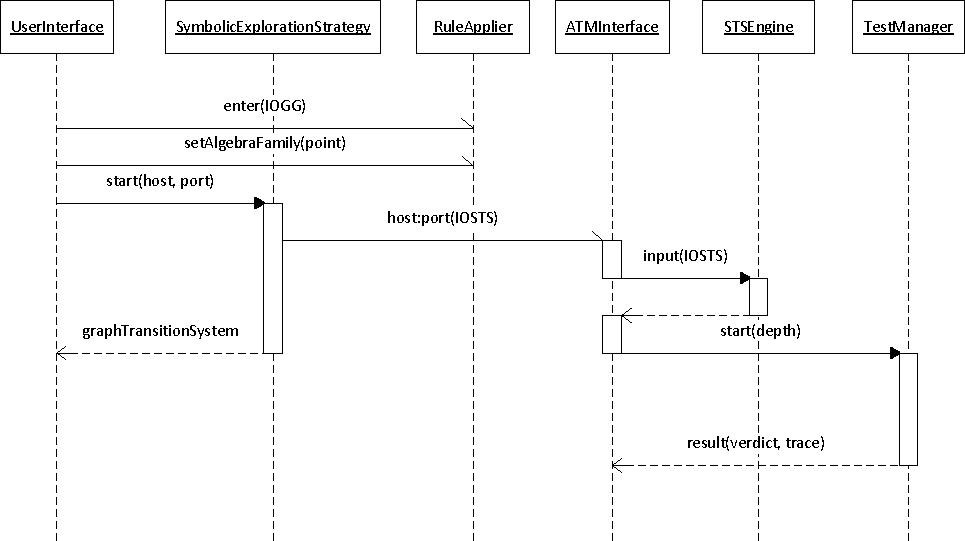
\includegraphics[width=\textwidth]{gratis_diagram.pdf}
  \end{center}
  \caption{GRATiS sequence diagram}
  \label{fig:tooling}
\end{figure}

\begin{enumerate}
\item The user enters an IOGG in the RuleApplier of the GROOVE tool. The input/output rules are defined by prefixing the given rule names with '?' and '!'. 
\item In the settings menu of GROOVE, the user sets the algebra family of the IOGG to to the point algebra, which is used by the RuleApplier.
\item The user selects the RemoteStrategy from the available strategies in GROOVE. This strategy gives input options to a host name and port number. The strategy is then started by the user. The communication between the RuleApplier and the strategy is omitted here, this is the same as in the GROOVE diagram. The result of the exploration is an IOGTS under the point algebra.
\item The RemoteStrategy creates an IOSTS in Java objects from this IOGTS with the method described in chapter~\ref{chapter:gg_to_sts}. It then creates a message with the IOSTS and sends this message to the ATMInterface
\item The ATMInterface receives the message and gives the IOSTS to the STSEngine.
\item The ATMInterface starts the testing with the default `depth' parameter; making this configurable is not implemented yet. The communication between the TestManager, STSEngine and Adapter is omitted here.
\item The TestManager returns the test results to the ATMInterface. The test results are stored in a database and are viewable by starting the user interface of ATM (ommitted here).
\end{enumerate}

\section{Description of added functionality}\label{sec:added_func}
This section covers in detail the added functionality to GROOVE and ATM. 

\paragraph*{GROOVE exploration strategy}
Figure~\ref{fig:esi-diagram} shows the class diagram of the added exploration strategy interface. The RemoteStrategy extends a \textit{SymbolicStrategy}. The SymbolicStrategy has a \textit{closing} exploration strategy, which is a strategy that explores all graph states and rule transitions, such as the BreadthFirstStrategy.

The user starts the RemoteStrategy with a host and port, as described above. This strategy starts a ClosingStrategy. This strategy explores the IOGG and notifies the remote strategy when there are no more rule transitions to explore. The SymbolicStrategy implements the method described in chapter~\ref{chapter:gg_to_sts} to build the IOSTS in Java objects using the explored IOGTS from the ClosingStrategy.
 
\begin{figure}[ht]
  \begin{center}
    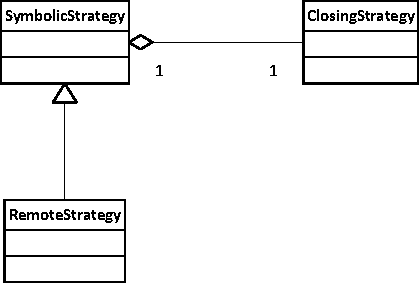
\includegraphics[width=0.35\textwidth]{strategy.pdf}
  \end{center}
  \caption{The class diagram of the exploration strategy interface}
  \label{fig:esi-diagram}
\end{figure}

\paragraph*{IOSTS in GROOVE}
Figure~\ref{fig:sts-diagram} shows the class diagram of the IOSTS in GRATiS. The IOSTS is composed of Location, SwitchRelation, Gate, Interaction- and LocationVariable classes. A Location object can be the start and target of any number of SwitchRelation objects. A SwitchRelation object has two Location objects; the start and target location. It also has one Gate object, which can belong to any number of SwitchRelation objects. A Gate object can have any number of InteractionVariable objects, but an InteractionVariable object belongs to only one Gate object. The IOSTS class has one singleton object, the RuleInspector, which contains the functionality of building guards and updates from rule graphs, i.e. the $\function_{\guard}$ and $\function_{\updateMapping}$ functions defined in~\ref{def:guard} and~\ref{def:um} respectively.

\begin{figure}[ht]
  \begin{center}
    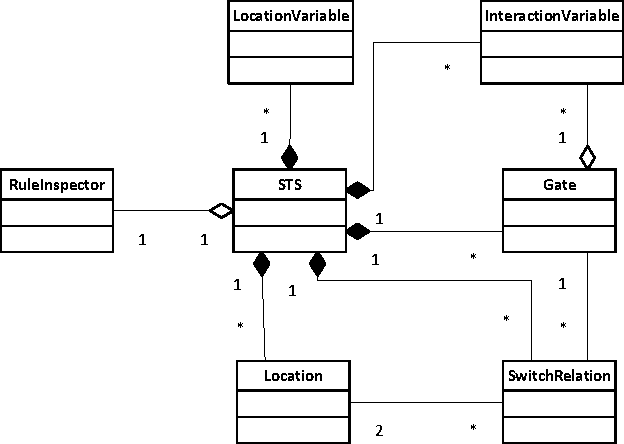
\includegraphics[width=0.5\textwidth]{STS.pdf}
  \end{center}
  \caption{The class diagram of the IOSTS in GRATiS}
  \label{fig:sts-diagram}
\end{figure}

Figure~\ref{fig:sts-objects} shows the object relations in accordance with the class diagram for the IOSTS in Figure~\ref{fig:example_sts}. Note that the links between the $\mathit{BoardGame}$ object and the the other objects are not drawn for the sake of clarity. Note that the created objects, inter-object relations and object parameters are in accordance with the method described in chapter~\ref{chapter:gg_to_sts}. The IOSTS itself is the composite object, which also holds the initialization function. The RuleInspector is not part of the IOSTS, therefore the Boardgame object does not show the relation with this object.

\begin{figure}[ht]
  \begin{center}
    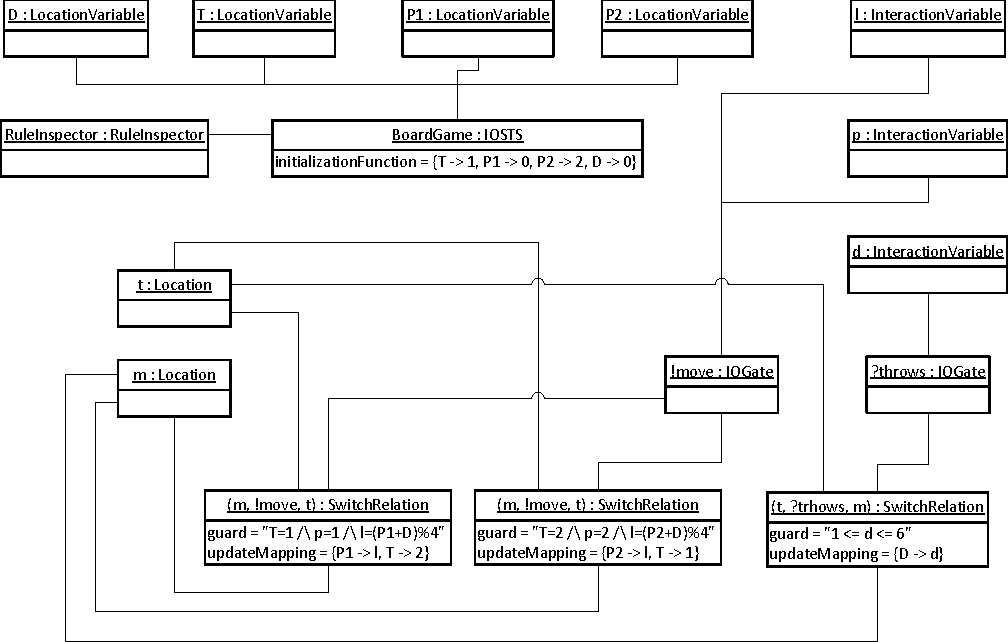
\includegraphics[width=0.8\textwidth]{STS_objects.pdf}
  \end{center}
  \caption{The object diagram of the IOSTS in Figure~\ref{fig:example_sts}}
  \label{fig:sts-objects}
\end{figure}

\paragraph*{GROOVE-ATM Interface}
The RemoteExplorationStrategy sends a HTTP POST request with the IOSTS in JSON format to the interface of ATM.
The ATM interface is one component in the Ruby on Rails framework. The interface is a controller in this Model-View-Controller framework. Controllers handle the HTTP requests given by the framework. The interface receives the IOSTS POST request, builds the IOSTS as Ruby objects and initiates the test using this IOSTS as model.